\documentclass{bhamthesis}
\usepackage[utf8]{inputenc}
\usepackage{url}
\usepackage{graphicx}
\graphicspath{ {images/} }
\usepackage[nottoc]{tocbibind}
\usepackage[toc, page]{appendix}
\usepackage[acronym, toc]{glossaries}
\setlength{\parindent}{4em}
\setlength{\parskip}{1em}
\title {Audit of SSH Client - PuTTY}
\author{Alok Vaidya (1624140)}
\date{August 14, 2017}

\makeglossaries
\newglossaryentry{rsa}
{
    name=RSA,
    description={A public key cryptosystem designed by Ron Rivest, Adi Shamir and Leonard Adleman}
}

\newglossaryentry{maths}
{
    name=mathematics,
    description={Mathematics is what mathematicians do}
}

\newglossaryentry{formula}
{
    name=formula,
    description={A mathematical expression}
}

\newacronym{rsa_ac}{RSA}{Rivest Shamir Adleman}

\newacronym{dh_ac}{DH}{Diffie-Hellman}
\newacronym{dsa_ac}{DSA}{Digital Signature Algorithm}
\newacronym{dss_ac}{DSS}{Digital Signature Standard}

\begin{document}

\maketitle
\tableofcontents
\begin{abstract}
The Secure Shell (SSH) protocol provides a mechanism to securely run network services over an insecure network. It is most commonly used for remote logins to shell accounts on Unix/Linux or other computer systems. PuTTY is an SSH client program running commonly on a Windows system providing users means to connect securely to a remote server. We performed a security audit of PuTTY with the purpose of finding vulnerabilities that, if exploited, would allow an attacker to compromise the security of an SSH connection. We primarily focused our attention on the Diffie-Hellman (DH) Key Exchange that leads to the establishment of a shared key that is used to encrypt all subsequent communication and on the Public Key Authentication mechanism used to authenticate the user to the server. We also analyzed randomness generation process, modular exponentiation implementations and supported legacy protocols. We performed a code review of the software in order to find possible vectors for known attacks and conclude that implementations of cryptographic primitives within the software employ all necessary safeguards to nullify such vectors.
\section*{Keywords}
SSH, PuTTY, Diffie-Hellman, Timing Attacks, RSA Blinding
\addcontentsline{toc}{section}{Keywords}
\end{abstract}
\section*{Acknowledgements}
This project reflects my efforts but it would not have been complete without the kind and gracious support of my supervisor Dr. David Oswald. I would like to take this opportunity to extend sincere thanks to him.\par
Dr.Oswald was always patient with my queries and provided constant supervision and guidance and necessary information to steer me to the completion of this undertaking. I am highly indebted to him for this. My efforts have also been influenced by discussions I have had the kind fortune to have with other professors and individuals each of whom provided valuable suggestions, insights and opinions, I am thankful to all of these individuals as well.
\addcontentsline{toc}{section}{Acknowledgements}
\chapter{Introduction}
\section{Overview}
In this chapter we provide a summary of the entire project to the audience. We begin by outlining the Secure Shell (SSH) protocol and the PuTTY Software and move forward by detailing the workings of Key Exchange and Public Key Authentication within the SSH protocol. We specify the goals and objectives we set out to achieve with this project. Lastly we explain the setup of the environment for the analysis we perform listing some of the tools we use.

\section{SSH and PuTTY}
SSH is a cryptographic network protocol used to provide secure network services over an unsecured network
\footnote{\url{https://en.wikipedia.org/wiki/Secure_Shell}}
The most common use of SSH is to remotely login to computer systems securely. Users on their computers use SSH clients that connect to an SSH server running on the server (remote) machine. PuTTY\footnote{\url{https://www.chiark.greenend.org.uk/~sgtatham/putty/}} is an SSH client software that runs most commonly on Windows systems. The PuTTY project among other programs includes Plink - a command-line interface to the PuTTY back ends and PuTTYgen - a RSA and DSA key generation utility. In the next section we introduce the workings of PuTTY with emphasis on the Diffie-Hellman (DH) Key Exchange and the Public Key Authentication sections.
\section{Diffie-Hellman Key Exchange}
To establish a session the SSH client initiates a connection to the SSH server and announces its own name and version along with the SSH version it implements. The server responds with a similar message identifying itself and its SSH version. Both the client and server must now establish a shared key that will be used to encrypt the messages for this session. This method to establish one-time session keys is known as Key Exchange. SSH clients and servers support multiple algorithms for Key Exchange \cite{rfc4253} such as DH, Elliptic Curve DH, RSA etc. For the specific purpose of this section we will assume that the client and the server have agreed upon the DH Group Exchange protocol.\par

Fig. 1.1 provides an overview of the DH Key Exchange process. Once the client and server have agreed upon the DH group parameters, the server sends the client suitable \textit{g} (generator for the DH group) and a corresponding prime \textit{p}. The client generates a secret exponent \textit{a} and computes \(e\ = \ g^a\ mod\ p\) and sends it to the server. The server computes a random exponent of its own, say \(b\) and sends \(f\ =\ g^b\ mod\ p\) to the client. In DH, \(a\) is known as Alice's (client's) secret and \(b\) as Bob's (server's) secret. On receiving \(e\) the server computes \(K\ =\ e^b\ mod\ p\)  i.e. \(g^{ab} \ mod\ p\) similarly the client computes \(K\ =\ f^a\ mod\ p\) i.e. \(g^{ba}\ mod\ p\). It's critical that both of the secret exponents \(a\) and \(b\) remain secret from an attacker. If either are somehow revealed, the attacker can compute the shared secret \(K\) by himself as both \(e\) and \(f\) are sent in plain text across the network. Once the client and the server both share a secret key, all subsequent communication is encrypted using the shared secret.
\begin{figure}[ht]
\caption{Exchange of messages during DH Key Exchange}
\centering
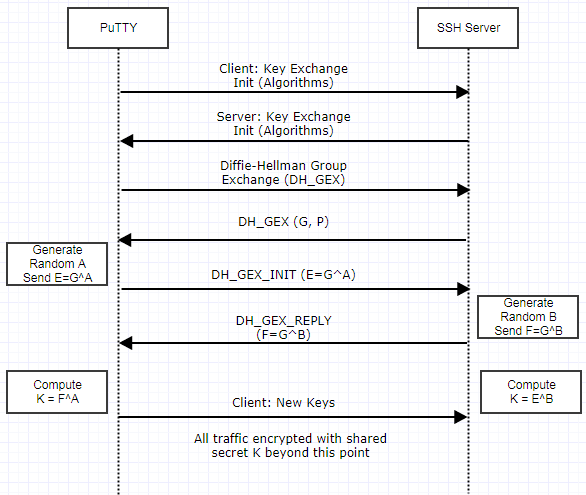
\includegraphics[width=0.72\textwidth]{SSH_DH_KEX.png}
\end{figure}
\section{Public Key Authentication}
A SSH server authenticates a user using either a password or a public key. When using public key authentication, the possession of a private key serves as authentication \cite{rfc4252}. The SSH client creates a signature using the user's private key. The server checks whether public key is a valid authentication mechanism for the user and that the signature verifies. If both conditions hold the access is granted. Fig. 1.2 offers an overview of the process\par
\begin{figure}[ht]
\caption{Public Key Authentication}
\centering
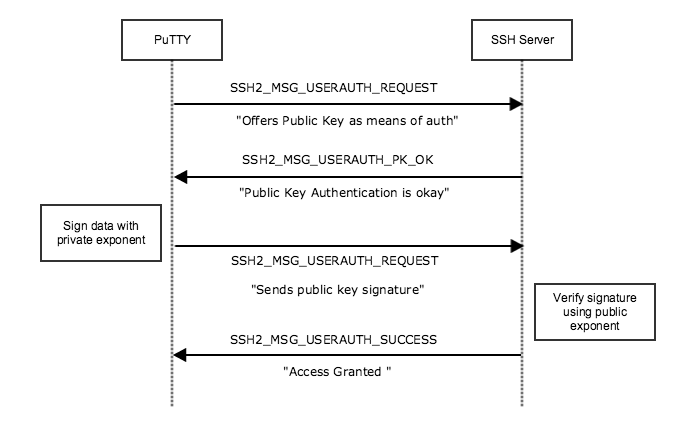
\includegraphics[width=1\textwidth]{SSH_PK_AUTH.png}
\end{figure}
\section{Objectives}
\par
Now that we have briefly described the DH Key Exchange and the Public Key Authentication processes of SSH, we move onto outlining the key objectives of the project.\par
As specified earlier, our primary objective is to find timing leaks in implementations of cryptographic primitives and in that regard we look closely at the implementations of DH Key Exchange and Public Key Authentication. Within these implementations the section of particular interest to us is the modular exponentiation operation. Both, the DH Key Exchange - during the computation of \(g^a\ mod\ p\) - and the Public Key Authentication - while creating the signature - use modular exponentiation. They use cryptographically sensitive data in their respective modular exponentiation and a timing leak in either of these operations could leak sensitive data. We analyze these operations in sections 3.2 "Timing Attack on DH Key Exchange" and 3.3 "Public Key Authentication Analysis".\par

Cryptographic primitives often require a random number generator that generates a random stream of bits. To ensure safety of sensitive data it is critical that this stream of bits be strictly random. To this end our next objective is to analyze and review the code responsible for randomness (a.k.a noise) generation. Additionally to test the statistical properties of the random numbers, we perform some common tests on them. Randomness generation analysis is covered in section 3.4 "Randomness Generation Analysis"\par
In line with our goal of a security audit of the entire software our next objective concerns performing an exhaustive analysis of all invocations of the modular exponentiation operation. This analysis aims to confirm that the data passed to each invocation is safe from tampering by an attacker. By manipulating data to such invocations information about sensitive data could be possibly leaked. Section 3.5 "Modular Exponentiation Analysis" describes this analysis.\par
Lastly we analyze and review the implementation of some of the legacy protocols that PuTTY supports. Section 3.6 "Legacy Protocol Analysis" provides the details of this.\par
\section{Environment Setup}
This section is supposed to acquaint the reader with the setup used for testing and measurements. We describe the audit process and methodology in the next chapter.\par

The source code of PuTTY was downloaded from the PuTTY homepage \cite{putty} and compiled on Windows 7 OS using Microsoft Visual Studio Community 2017. It provides solutions for all PuTTY projects including those mentioned in section "SSH and PuTTY". Compiling a solution for a project renders an executable. For debugging and flow control analysis, PuTTY was run in debug mode in Visual Studio. For automated measurements a Plink executable with extensions to code was created. This executable was then invoked from a Java program for multiple measurements. For both debugging and automated measurements a Bitvise SSH Server running on the same host, was used as a server. Alternatively for simulating messages across a network an OpenSSH server running on a Raspberry Pi was used \footnote{Refer Appendix D: "Software and Tools"}.
\chapter{Methodology}
\section{Overview}
The security audit involved analyzing different aspects of the software. To accomplish these analyses several different methodologies were adopted. This chapter briefly explains each one of them.
\section{Code Review}
To perform each analysis, to either rule out the possibility of an attack or to accept it and then attempt to carry out the corresponding attack a deep understanding of the code was required in terms of control flow and data manipulation. As a result code review played a critical role in each of the analysis.
\section{Custom Code}
Specific portions of code were amended to include custom code to make precise timing measurements, manipulate, test and log data values, run desired sections repeatitively etc.
\section{Literature Review}
A review of published literature related to Timing Attacks, Attacks on Diffie-Hellman and RSA/DSA signing provided a sense of possible exploits and attack vectors. Consequently this informed what to look for in a code review. With regards to Randomness Generation, published papers were used to inform our view on what test suites to use, standard testing practices, sample sizes etc.
\section{Randomness Test Suites}
In addition to the code review of the Randomness Generation Process, we performed relevant tests on generated random data. Results from such tests offer us more insight on the Random Number Generator (RNG). Our choice of tests was informed by multiple sources on the internet, reputed websites offering RNG services and published papers.
\chapter{Security Analysis}
\section{Overview}
This chapter summarizes our security analysis on different aspects of the PuTTY code. We begin by analyzing a timing attack on the DH Key Exchange. The intent of this attack is to reveal the DH secret exponent for the client. The secret exponent is generated using random data from the RNG and hence the properties of the RNG too are critical for our analysis. We take a look at both the generation process for the secret exponent later in this section and the application-wide randomness generation process later in this chapter. We conclude the section analyzing yet another important characteristic of the secret exponent - its bit-length. We look at potential attacks on exponents with shorter bit-lengths. \par
Next we attempt a timing attack on the public key signing operation within the public key authentication mechanism with the intent to reveal the private exponent of the key. We briefly visit the public key authentication process, we explain causes of timing differences in the signing operation, we explain details of how these timing differences might be exploited to carry out an attack, we discuss a safeguard that PuTTY employs against this attack and finally describe an artificial attack that may be carried out. \par
The next section describes the randomness generation process implemented by PuTTY. We gather such randomness and subject it to a few tests and report on the results. \par
In the next section we conduct a security analysis of individual invocations of the modular exponentiation operation with the intent to find invocations on which an attacker may be able to manipulate the arguments and exploit timing differences to reveal sensitive data.\par 
Finally we analyze a legacy key exchange protocol supported by PuTTY intending to find vulnerabilities in its implementation.
\section{Timing Attack on DH Key Exchange}
In a DH Key Exchange between a client and a server that culminates in a shared secret, both the client and the server are required to perform a modular exponentiation operation individually with a secret exponent. This modular exponentiation operation may be vulnerable to timing attacks and an attacker could be able to find the secret exponent by carefully measuring the timing required to perform operation \cite{kocher96}.\par
We explored the possibility of this attack being carried out on the DH modular exponentiation implementation within PuTTY by reviewing the relevant code sections. Instead of using the same exponent in each invocation of the Key Exchange, a new random exponent, is generated every time. If this is so, the attack does not work \cite{kocher96}.
\subsection{Secret Exponent Generation}
During each DH Key Exchange PuTTY generates a random exponent. The number of bits in the exponent depends on the number of bits desired in the key to be established through the DH Key Exchange. The number of bits in the exponent is set to twice as those desired in the key. As we will see in the next section this bit-size of the exponent paired with a safe prime provides the necessary safety.\par
The figure below explains how PuTTY arrives on the random exponent.
\clearpage
\begin{figure}[ht]
\caption{Random Exponent Generation}
\centering
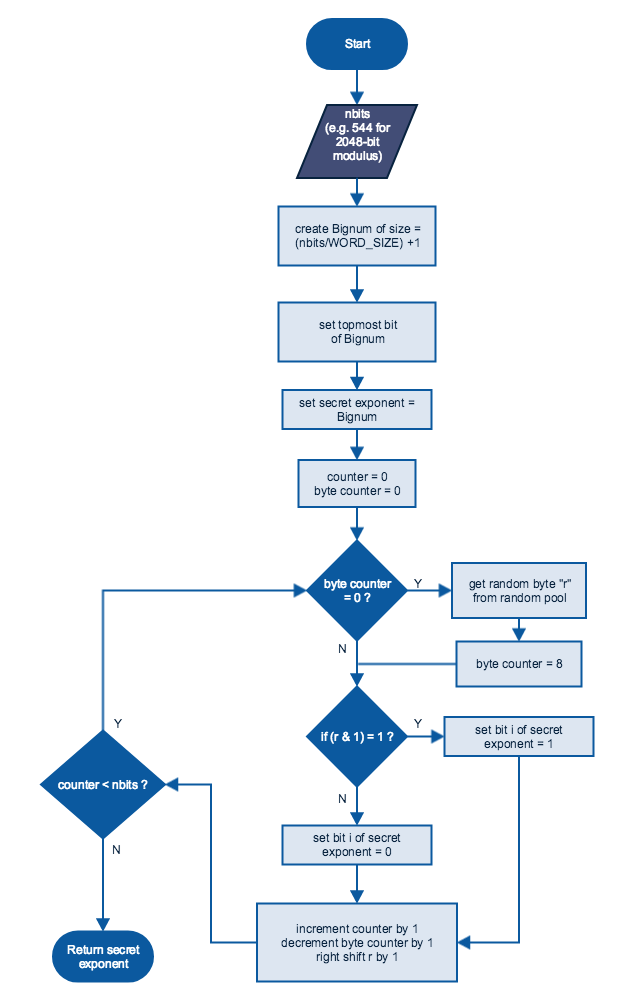
\includegraphics[width=0.65\textwidth]{Rand_Expo.png} 
\end{figure}
\subsection{Attack on Short Exponents in DH}
In \cite{oorschot96} the authors present a technique that can be used to recover short exponents (160-bit exponents with 1024-bit primes). To explore the possibility of this attack, we analyzed the length of the exponents used by PuTTY in its implementation. The bit-length of the exponent is dependent on the DH group in use. For DH Group 1 with 1024-bit primes, which has the lowest bit-lengths, the length of the exponent is 384 bits. For DH Group Exchange, which is the default when DH is used, wherein the client specifies to the server a minimum, a maximum and a preferred length of bits for the prime, the exponent is 544 bits. So even the shortest exponent supported by PuTTY is sufficiently long. These exponents together with safe primes, which SSH mandates, precludes the above attack.
\section{Public Key Authentication Analysis}
This section analyzes if we are able to exploit any timing attacks within the public key authentication process. The intent is to be able to reveal the user's private key.
\subsection{Public Key Authentication Process}
As mentioned in section 1.4 "Public Key Authentication", in public key authentication the possession of a private key serves as the authentication for the user. In this section we explain the process in detail and then look at the part we are most interested in i.e. the signing with the private key.\par
\begin{figure}[ht]
\caption{Exchange of messages during Public Key Authentication}
\centering
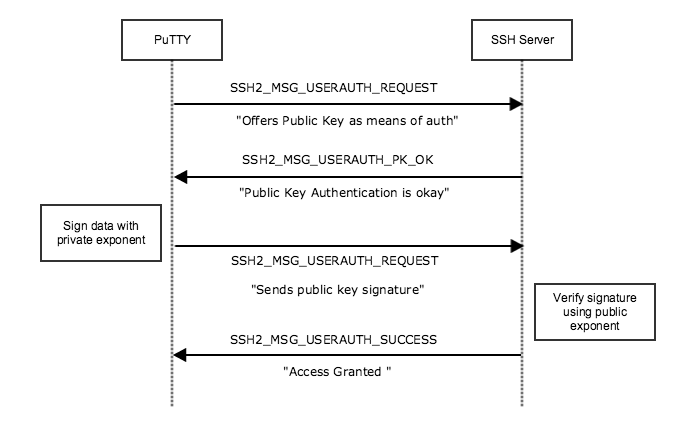
\includegraphics[width=1\textwidth]{SSH_PK_AUTH.png}
\end{figure}
The image above provides an overview of the process. The client requests the server to be allowed to use public key as an authentication mechanism. The server responds positively if the user may be allowed to use public key or negatively otherwise. On receiving a positive response the client proceeds to generate and send a signature to the server which is then verified by the server and depending on whether the verification succeeds the server grants access to the user.\par
In the procedure explained above we focus our attention on the operation that generates a signature using the user's private key. The signature is generated over a set of data that includes - the session identifier, hex code identifying the request,user name, service name, the string \textit{"public key"}, a boolean value \textit{TRUE} identifying that this message contains the actual signature, public key algorithm name and the public key to be used for authentication. To be precise the signature is actually generated over a hash of the above values.

\subsection{RSA Blinding}
To explore the possibility of a timing attack on the public key signing operation we review the relevant code sections. The file \textit{sshrsa.c} deals with the implementation of the RSA protocol and the public key signing operation is incorporated within the function \textit{rsa2\_sign}. Reviewing the code in this function we observe that PuTTY employs RSA Blinding during the exponentiation to prevent an attacker to be able to draw any correlation between the timing of the operation and the exponent used. Remember the exponent used is the private key (the private exponent of the RSA key). This essentially safeguards against the possibility of a timing  attack. The next paragraph discusses the implementation of the blinding process and how it protects against the attack.\par
We explain how RSA blinding is implemented and how it protects against a timing attack. Let's assume \(x\) is the base or the hash value of data to be signed, \(d\) is the private exponent of the key and \(p\) the modulus. The signature is computed thus - signature \(s\ =\ x^d\ mod\ p\). When this operation is performed by itself minor timing differences in the operation shall reveal the private exponent of the key. We generate a random, say \(y\) and instead of computing  \(x^d\ mod\ p\) we compute \((x*y)^d\ mod\ p\). Note that, \((x*y)^d\ mod\ p\) = (\(x^d\ mod\ p\)) * (\(y^d\ mod\ p\)). Hence, we instead compute the signature thus \(s\ =\ ((x*y)^d\ mod\ p\))/(\(y^d\ mod\ p\)). The benefit this has is that because the attacker has no knowledge of either \(x\) or \(y\) (\(y\) is generated randomly using sound randomness), he is unable to correlate the timing of the operation with the value of \(x\) which precludes the timing attack. Please note there have been attacks developed quite recently that can still work even if the software employs blinding. This attack is termed as the "Cross-correlation Attack". Please refer section 5.4 "Cross-correlation Attack" \cite{vadnala} of chapter 5 "Further Work".
\subsection{Random Generation for Blinding}
The random number (\(y\) above), does not come from the Random Pool maintained as a main source of randomness by PuTTY. Instead the random for the blinding process is generated by hashing different values with the private key.\par
The process begins by choosing a number of the length of the modulus, the position of the top most set bit is found and all lower bits are randomly set travelling downwards from that bit. Then PuTTY proceeds to hash different things with initial value, lastly the private exponent of the key is hashed with it.\par
The random is chosen uniformly from the range \(2.. (modulus - 1)\). If the random chosen is greater than the modulus then a new random computed instead of just reducing the random mod \(n\), to avoid any attacks making use of the uneven distribution within the said range that would arise from just reducing the number mod \(n\).
\subsection{An Artificial Attack}
We seek to know whether a timing attack is possible on the signing operation without the blinding employed. To explore this, we first amend the source code to completely strip off the blinding. In addition to stripping off the blinding code, we also comment out the code for the random generation. In effect we are reverting the code back to performing the simple computation for the signature \(s\ =\ x^d\ mod\ p\).\par
We explore the possibility of applying the attack from \cite{brumley} on the public key signing process after removal of the blinding code. The paper discusses remote attacks on RSA decryption in OpenSSL\footnote{\url{https://www.openssl.org/}}. Decryption is performed by the private exponent of the key as is the signing (our case). PuTTY, like OpenSSL, uses Chinese Remainder Theorem (CRT) to perform the exponentiation for the signing process. Using CRT the exponentiation \(s\ =\ x^d\ mod\ p\) is computed in two steps, first evaluate \(s_1\ =\ x^{d_1} \ mod\ p_1\) and \(s_2\ =\ x^{d_2} \ mod\ p_2\) (Here, \(p\ =\ p_1\ *\ p_2\) and \(d_1\ and\ d_2\) are pre-computed from \(d\)), second to combine \(s_1\) and \(s_2\) using CRT to get \(s\). A timing attack can expose the factors \(p_1\) and \(p_2\). Revealing the factors effectively reveals the private exponent \(d\) (\(d\ =\ e^{-1}\ mod\ ({p_1}\ -\ 1 )\ ({p_2}\ -\ 1)\) , \(e\) is the public exponent of the key). \par
The authors in \cite{brumley} mention two different sources of timing differences originating in the modular exponentiation process. The first difference in timing arises from the use of Karatsuba or ordinary multiplication for multiplication in the exponentiation operation. Karatsuba being faster runs in shorter time. The second difference originates from what is called as an "Extra Reduction" at the end of Montgomery reduction. Montgomery reduction transforms a reduction modulo \(p\) (the modulus) into a reduction modulo some power of 2 which can be efficiently implemented as a series of operations in hardware. At the end of the reduction the final result is checked to see if it is greater than the modulus \(p\). If it is, than the result is reduced modulo \(p\) to ensure the result is in the range [\(0\ -\ p\)). This step is named as the "Extra Reduction" and causes timing differences in different inputs. The probability that an Extra Reduction will be required increases as the base \(x\) approaches the modulus \(p\) from below, at values of \(x\) that are multiples of \(p\) the probability drops sharply to zero. If the timing measurements are recorded onto a graph the increasing time for the operation  as \(x\) approaches \(p\) from below followed by sharp drops at \(x\) equal multiples of \(p\), form peaks on the graph that help us make estimations at the values of \(p\). We can then by making educated manipulations to the value of \(x\) figure bits of \(p\).
\subsection{PuTTY's Exponentiation Implementation}
To explore the possibility of carrying out this attack on PuTTY's implementation, we begin by reviewing implementation of the exponentiation operation. We investigate whether the two above mentioned sources of timing differences do indeed exist in PuTTY's implementation. If they do we can proceed to perform a similar attack from \cite{brumley}.\par
PuTTY implements both the Karatsuba and the ordinary multiplication algorithm for performing the multiplications resulting from the exponentiation. However it exercises a  threshold on the size of the modulus of the exponentiation to decide whether or not Karatsuba should be used. This threshold defined in the file \textit{sshbn.c} is 50 words (50 * 32 = 1600 bits on 32-bit platforms and 3200 bits on 64-bit platforms). If the modulus is smaller than 50 words ordinary multiplication algorithm is used. With CRT in use this threshold restriction applies not to the original modulus but to \(p_1\) and \(p_2\), the moduli that apply to the two split exponentiations performed by CRT, remember \(p\) = \(p_1\) * \(p_2\). Since the most common bit-length for an RSA key modulus is 2048, the factors \(p_1\) and \(p_2\) are typically half the size or 1024 bits in length. Even with a 3072-bit modulus for RSA, the factors are typically 1536 bits in length. As a result PuTTY almost always ends up using only the ordinary multiplication algorithm and almost never using Karatsuba. This results in one of the sources of timing differences as identified in \cite{brumley} not being so in PuTTY.\par
\subsection{Extra Reduction in PuTTY}
As mentioned above the second difference in timing originates from the Extra Reduction at the end of a Montgomery reduction. The differences in timing caused by the Extra Reduction can be exploited to carry out an attack as described in \cite{brumley}.\par
Remember that CRT splits the exponentiation operation \(x^d\ mod\ p\) into two exponentiation operations with the factors of \(p\ =\ p_1\ *\ p_2\) as moduli. So the timing attack above should recover both the factors \(p_1\)  and \(p_2\) for us. Once the factors are known we can get the private exponent as follows:\\
    \(d\ =\ e^{-1}\ mod\ ({p_1}\ -\ 1 )\ ({p_2}\ -\ 1)\), \(e\) is the public exponent.
\section{Randomness Generation Analysis}
Implementation of cryptographic primitives requires the generation of randomness. This section explains the process and flow of randomness generation within PuTTY. We identify the sources for the randomness and in our endeavour to establish the properties of the randomness generated, we gather the random data and subject it to to some standard tests.
\subsection{Randomness Generation Process Overview}
PuTTY maintains a pool of size 1200 bytes of random generated data, from which it hands out bytes of data to processes that request it. This pool of data is filled at start-up from noise generated from various sources such process listings, local-time, random files on search paths and other environmental noise. A seed from a seed file that is maintained by PuTTY in the Windows Registry is also used. This process is called "heavy noise generation" and occurs only once in one invocation of PuTTY.\par
This generated random data then undergoes a process what PuTTY calls "Random Stir". This random stirring involves two passes of SHA (Secure Hash Algorithm) Transformation where SHA is operated in CFB (Counter Feedback) mode and the output is repeatedly fed back to the SHA digest.\par
Random noise is generated in the background every 5 minutes and added to a buffer known as "incoming buffer". When this buffer gets full, the contents are added to another holding area called simply as "incoming" where it will be held to be used for "stirring" the pool when required.\par
Data from this random pool is handed out to a requesting entity such as PuTTY's implementations of cryptographic primitives. PuTTY maintains a pointer to the pool and advances this pointer as it hands out random data until the pointer reaches the end of the pool at which point the pool is stirred again using noise generated so far from the environment in the incoming buffer and the pointer is reset to its starting position.\par
\begin{figure}[ht]
\caption{Randomness Generation Process in PuTTY}
\centering
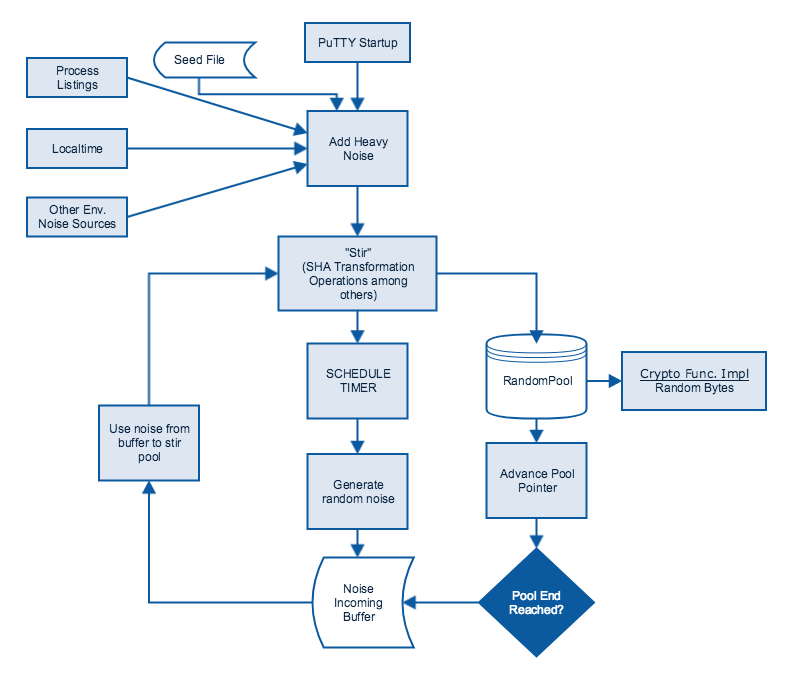
\includegraphics[width=1\textwidth]{NG.png}
\end{figure}
\subsection{Test Data Collection}
Data was collected for testing in two primary ways. A file logging utility within the \textit{sshrand.c} file - the program primarily responsible for generation and maintenance of randomness within PuTTY. This utility was invoked every time a block of random data was about to be added to the random pool. It logged the data block as it is into a file. This generates raw binary data in the file. The second method of collection followed a more traditional approach, one that protocol implementations follow within the code. In this method we make use of the function call \textit{random\_byte()}. This function returns a single byte of data as a number from 0-255. we logged this too in a file for later analysis.\par
Randomness Tests require a significant amount of data to be present in the file they are to test as more data typically results in better accuracy. To generate enough data one of two techniques was used. Either to keep the application running in the background so that it keeps generating randomness according to its schedule every 5 minutes or call the \textit{random\_byte()} function in a repeated loop. Clearly the earlier mechanism is time consuming and requires some interaction on the established connection for PuTTY to keep generating fresh randomness. Even then this requires too long to generate data sufficient to be used in a test with reliable results. The latter mechanism generates sufficient data quickly but may not result in good randoms (Generally it takes time for data with sufficiently high entropy to be generated from environmental sources).
\subsection{Randomness Tests}
Here in this section we study the properties of the random numbers we have generated and also apply standard tests to them. We measure the statistical properties on a sample of 10,000 numbers of one byte each [0-255]. \cite{randeval} and \cite{foley} among other sources were used to advise on what statistical properties to report on, what tests to perform, how tests should be applied and how results should be interpreted.\par
The table below summaries the statistical properties of the numbers. \par
\begin{figure}[ht]
\caption{Summary Statistics}
\centering
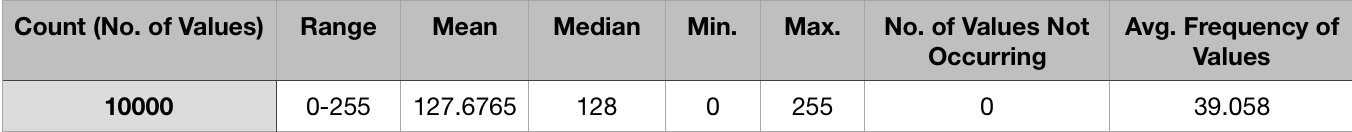
\includegraphics[width=1\textwidth]{stat_summary.png}
\end{figure}
Count is just the total number of values in the sample, since the randoms are byte-sized the range is 0-255, a Mean of 127.67 suggests the data is quite uniformly distributed within the range, there were no values from the range that did not occur in the sample and the average frequency of values is 39.058 which in a sample of 10,000 values with 256 unique values seems accurately representative.\par
Exploratory Data Analysis techniques help us get better acquainted with the data \cite{foley}. The two charts we present next should provide a visual measure of how random the data is. The X-Y scatter chart (Figure 3.5) exhibits a uniform distribution as suggested by the Mean.
\begin{figure}[ht]
\caption{X-Y Scatter Chart}
\centering
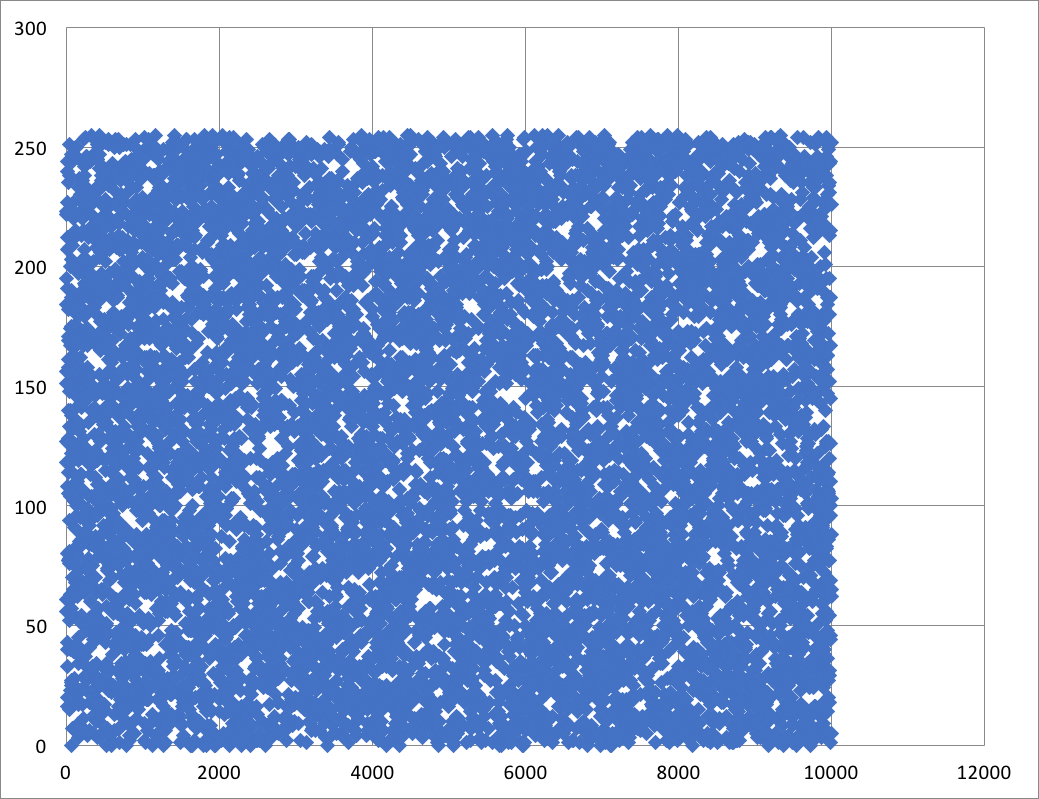
\includegraphics[width=0.8\textwidth]{xyscatter.png}
\end{figure}
The Bar Chart (Figure 3.6) shows frequencies for each of the values with a trend line across the graph nearing 40 which as mentioned above seems appropriate considering the number of values and the sample size.\par
\begin{figure}[ht]
\caption{Value Frequency}
\centering
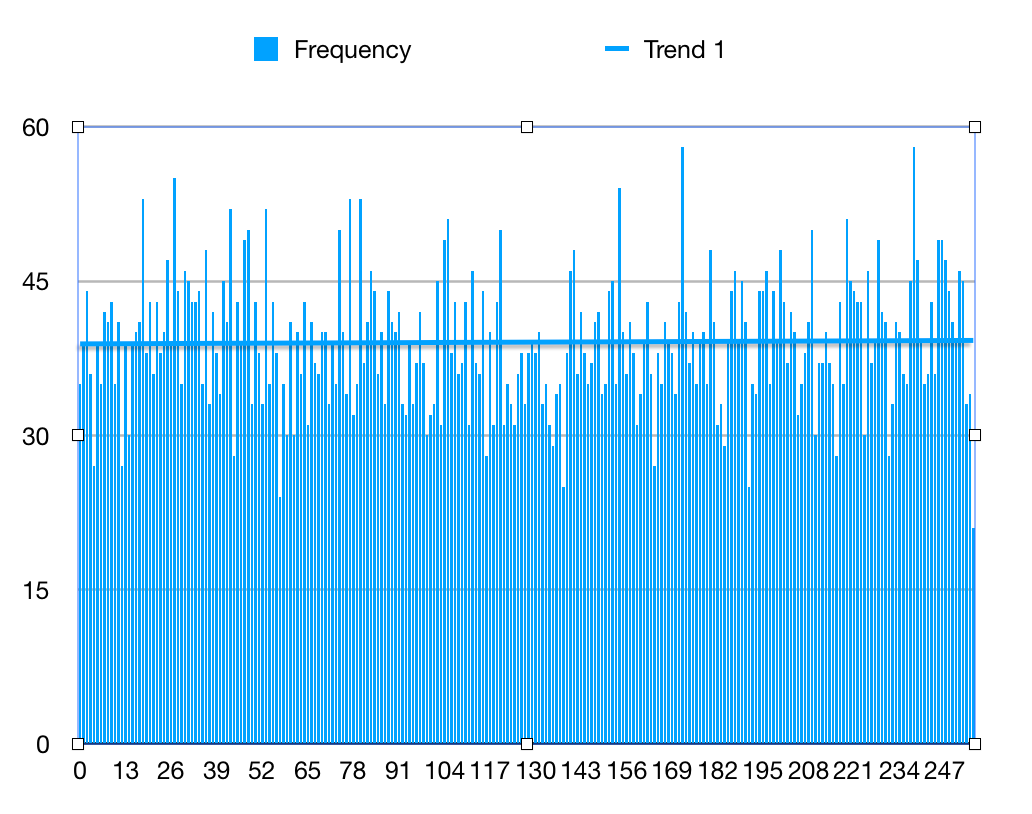
\includegraphics[width=0.8\textwidth]{barchart.png}
\end{figure}
\clearpage
Next, we present the results of running our random numbers through tests. 
\subsection{A Note on Sequence Generation}
As mentioned earlier in the section 3.4.1 "Randomness Generation Process Overview", PuTTY periodically generates randomness from external sources and adds it to the random pool. Further it has been observed that this process of randomness generation is sped up if the communication channel to the server is kept busy i.e. either party sends information to the other. If a channel is just left open without any information exchange taking place it takes a couple hours to generate 100KB of random data. Since more data is required for testing that too in a shorter time period, we induce the information exchange ourselves. We do this by opening an SSH connection to the server and searching recursively on the root directory for files with common name prefixes (such as "win*" on a Windows Server). This not only causes the server to send all information on "hits" from the search to the client, but because the name prefix is common and because we search recursively on root directory the search continues for a long time and the server keeps sending ongoing search data to the client. As a result of this enough random data is generated which we log to our file as sample data.\par

\subsection{ENT Test}
ENT from fourmilab\footnote{\url{http://www.fourmilab.ch/random/}} applies a variety of tests to a sequence of bytes and reports on the results. We ran ENT against files of increasing size containing random data in raw binary format generated from PuTTY's random pool. Finally we ran ENT against a file of 16,384 bytes of raw data generated from Random.org\footnote{https://www.random.org/ - Random.org uses atmospheric noise to generate randomness.} as a comparative measurement.\par
\begin{figure}[ht]
\caption{ENT Test Results: Sample File 1}
\centering
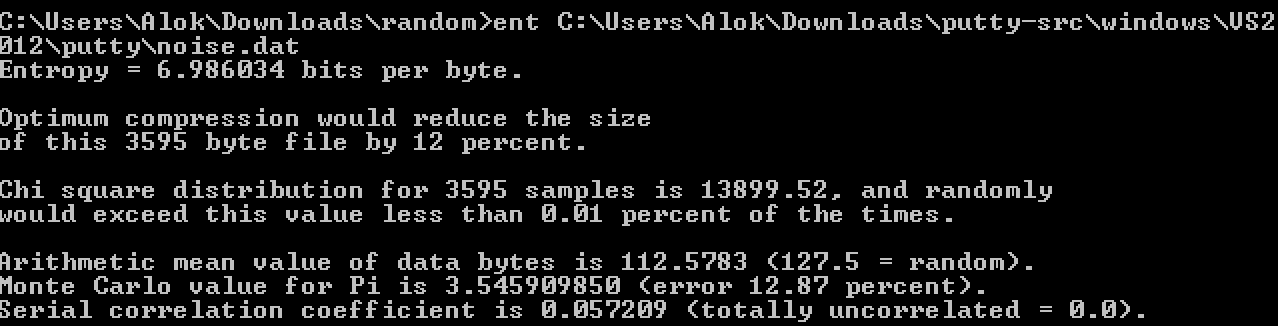
\includegraphics[width=1\textwidth]{ENT-Test1.png}
\end{figure}
\clearpage
\begin{figure}[ht]
\caption{ENT Test Results: Sample File 2}
\centering
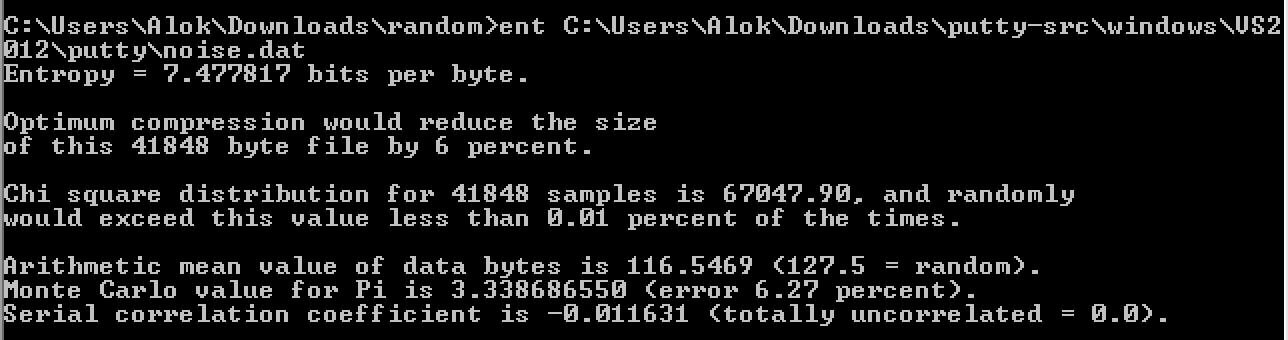
\includegraphics[width=1\textwidth]{ENT-Test2.png}
\end{figure}
\begin{figure}[ht]
\caption{ENT Test Results: Sample File 3}
\centering
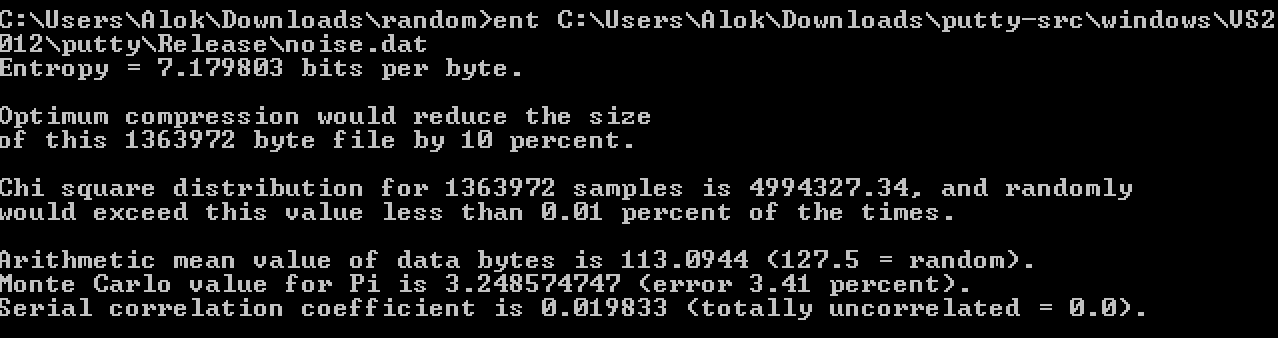
\includegraphics[width=1\textwidth]{ENT-Test3.png}
\end{figure}
Information Entropy\footnote{\url{https://en.wikipedia.org/wiki/Entropy_(information_theory)}} provides an indication to the amount of information in the data. It is used as a preliminary test of randomness. Typically random data will have high entropy. It can be seen in the results of the three samples above that the entropy of the data increases as bigger samples are generated. One issue believed to be present with PuTTY's random number generator is as more and more samples are generated in relatively shorter periods of time, as is the case typically when big samples are to be generated for testing, the entropy falls. This could be as a result of not enough entropy available from the source in the first place. This effect is also typically observed with Unix's \textit{/dev/random}.\par
The Chi-Square distribution is calculated for a sequence of bytes and reported as an absolute number and a percentage which indicates how frequently a truly random sequence would exceed the value calculated. When the percentage is greater than 99\%
or less than 1\% the sequence is, according to ENT's maker fourmilab.ch, "almost certainly not random". For all of the samples ENT reports the sequences not to be random. This finding is somewhat surprising as we test both small and large sequences. This though could again be due to the sequences generated in a shorter period of time, not allowing the source to collect enough entropy.\par
Arithmetic Mean is simply the average of the sequences which, all of them being byte values [0-255] should be 127.5. The three samples have averages approaching that value but not close enough, possibly suggesting want of bigger samples.\par
The Monte Carlo value for \(pi\) clearly approaches the actual value as the samples become bigger suggesting issues with size of data than the data itself.\par
In all of the samples, successive data values show no correlation between them, which suggests good randomness.\par
Finally we present ENT results for a sample of sequences generated by Random.org.
\begin{figure}[ht]
\caption{ENT Test Results: Sample from Random.org}
\centering
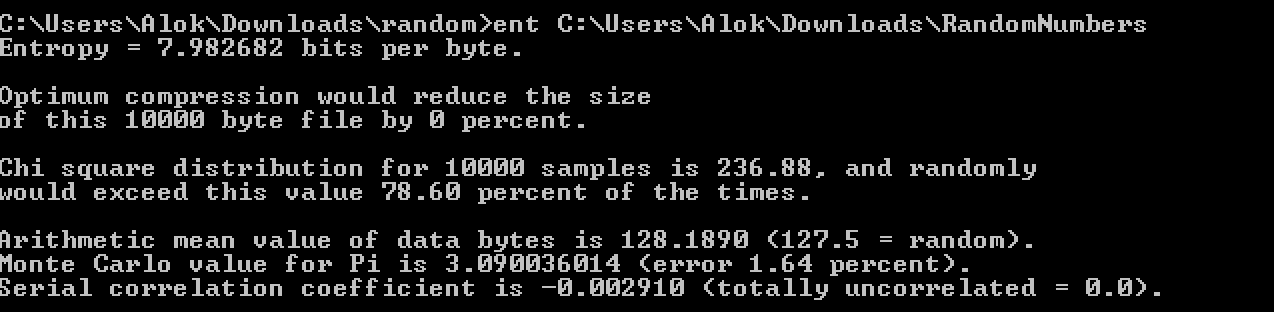
\includegraphics[width=1\textwidth]{ENT-Test-RandomORG.png}
\end{figure}
\section{Modular Exponentiation Analysis}
We analyze whether an attacker, by being able to manipulate arguments passed to a modular exponentiation invocation carry out timing attacks to reveal cryptographically sensitive data values.
\subsection{Modular Exponentiation Review}
PuTTY implements a modular exponentiation operation that is invoked by implementations of primitives such as RSA, DSS, ECC and DH. We exhaustively review each of these invocations to study and analyze the source of the arguments passed to the operation with the aim to discover whether an attacker would be able to tamper with the arguments. The ability to manipulate data arguments to the modular exponentiation algorithm would give an attacker the ability to measure the slight timing differences in the runtime of the operation as a result of different inputs.\par
The modular exponentiation operation in PuTTY is called \textit{modpow} and is invoked with three arguments - base, exponent and the modulus. We list each invocation and analyze it here.\par
\clearpage
\begin{enumerate}
    \item \textbf {Diffie-Hellman Implementation}
    In DH the \textit{modpow} operation is invoked twice. Once for the computation of \(e\ =\ g^a\ mod\ p\) and once for computing the shared secret \(K\ =\ f^a\ mod\ p\). While both invocations include arguments that are sourced over the network - \(g\) and \(p\) in the first and \(f\) in the second invocation - it does not make sense for an attacker to tamper these. An attacker in this case, would be acting as a man-in-the-middle between the client and the server and would have a DH shared key negotiated both with the client and the server individually. We can conclude that both these invocations are safe against possible tampering from an attacker.
    \item \textbf {DSA (Digital Signature Algoritm) Implementation}: 
    In DSA implementation the \textit{modpow} operation is invoked a total of four times - twice in the DSA signature verification - computing \(g^{u_1} \ mod \ p \) and \(y^{u_2}\ mod \ p\), once in DSA public key creation and once in DSA signing - computing \(g^k \ mod \ p\).\par
        \begin{enumerate}
        \item \textbf \underline{DSA Signature Verification}    \begin{itemize}
            \item {\(g^{u_1} \ mod \ p \)}: Both \(g\) and \(p\) come from the DSA as negotiated parameters. \(u_1\) is computed internally from other values.
            \item {\(y^{u_2} \ mod \ p \)}: \(y\ = \ g^x\ mod \ p\) and \(p\) comes from DSA as negotiated parameter. \(u_2\) is computed internally from other values.
         \end{itemize}
        The attacker cannot manipulate \textit{modpow} arguments to exploit any timing attacks.
        \item \textbf \underline{DSA Public Key Creation}
        \begin{itemize}
        \item
        The \textit{modpow} operation is called within the public key creation operation to verify \(y \ =\ g^x \ mod \ p\). Parameters \(g\) and \(p\) are DSS parameters and \(x\) is the secret exponent generated randomly internally. The attacker cannot manipulate any of these arguments to his benefit.
        \end{itemize}
        \item{DSA Signing}
        \begin{itemize}
        \item
        Used to compute \(g^k \ mod \ p\) where \(g\) and \(p\) are DSA parameters and \(k\) is generated randomly. Since none of the parameters come from external sources the attacker cannot manipulate them.
        \end{itemize}
        \end{enumerate}
    \item \textbf{ECC (Elliptic Curve Cryptography) Implementation}:
        In the ECC implementation \textit{modpow} is used thrice, once in point verification and twice in for Edward curve.
        \begin{enumerate}
            \item {Point Verification}:
            Computation of \(x^3\ mod\ p\). Parameters are either ECC parameters or are computed internally elsewhere within the calling operation.
            \item{Edwards Curve}:
            Both invocations for the Edwards Curve are heavily dependent on arguments that are computed elsewhere in the calling operation. No arguments have external sources.
        \end{enumerate}
        The attacker does not have an option to tamper with arguments to attack the \textit{modpow} operation to reveal any sensitive values.
    \item \textbf{RSA Implementation}: For RSA implementation the \textit{modpow} operation is invoked a total of five times - once for encryption with the RSA public key, twice from within CRT (Chinese Remainder Theorem) optimization to compute the result modulo the two moduli \(p\) and \(q\), once for verifying a RSA host key for the server and lastly for encryption in RSA Key Exchange.
        \begin{enumerate}
            \item{RSA Encrypt}: The base is the SSH session-key, stored internally, the exponent is the key's public exponent, the modulus is the key's modulus (not secret). Since the public key is assumed to be installed safely prior to this operation, we conclude that the attacker cannot manipulate arguments to his benefit.
            \item{CRT Optimization}: In both the modular exponentiation calls all the arguments are sourced either from within the calling operation itself or from a calling function one level higher, but since the arguments aren't influenced by external values, the attacker as no possibility of being able to manipulate the arguments.
            \item{Signature Verification}: This invocation of \textit{modpow} is within the RSA host key verification. Even if the attacker can manipulate the parameters to the operation such as the signature it won't be of any benefit to him as the only data that can be revealed (even if) is the signature that he himself sent us, the other parameters such as the key exponent and the modulus are public.
            \item{RSA Key Exchange Encrypt}: All data arguments have source internal to PuTTY, so the attacker cannot tamper with the data in any way.
         \end{enumerate}   
\end{enumerate}    
\section{Legacy Protocols Analysis}
In this section we examine legacy protocols supported by PuTTY with the aim to find any possible vulnerabilities in their implementation.
\subsection{Motivation}
Protocols that are old and aren't mainstream anymore may have vulnerabilities that are overlooked because the portion of code dealing with them is rarely used, or because such code would not be tested nearly as heavily as the code dealing with default, most commonly used protocols, or simply because a new attack makes the code vulnerable. Such protocols maye be supported just because of compatibility issues with genuine old servers. Even though these protocols aren't default, this won't stop an attacker with a malicious SSH server to make them be chosen by downgrading the list of supported protocols on his malicious server. Once the protocol is in use he can exploit any existing vulnerability.
\clearpage
\subsection{Analysis of Diffie-Hellman Group 1}
For Key Exchange PuTTY supports DH Group 1 which is a very weak DH group of 1024-bits. We must note that PuTTY does warn the user against selecting this protocol as is evident from the image below.
\begin{figure}[ht]
\caption{Warning against use of weak DH Group for Key Exchange}
\centering
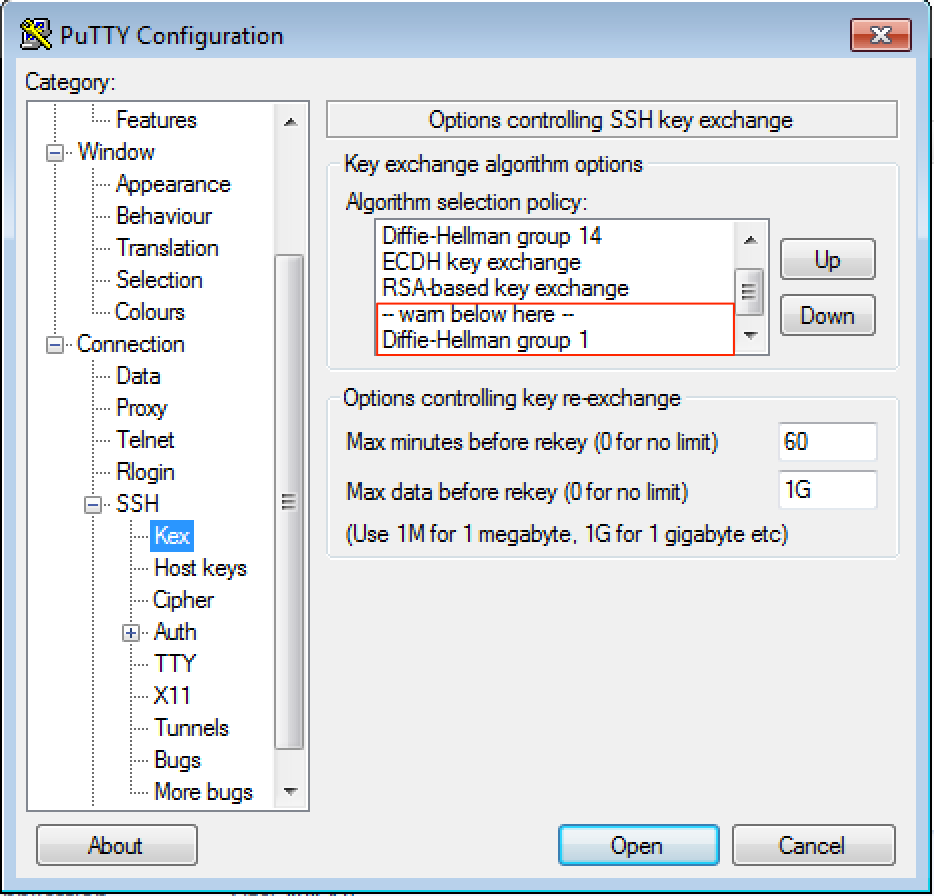
\includegraphics[width=1\textwidth]{legacy.png}
\end{figure}
We traced the control flow for this protocol and reviewed the code in use. Having a 1024-bit group, it is vulnerable against nation-states adversaries against the LogJam attack \cite{adrian}. This, understandably is not a vulnerability in PuTTY. The secret exponent (client's secret) under this group is significantly shorter (384-bits) than the typical value (544-bits). Upon inspection though we find that the code segment used is the same as that for higher stronger groups. Only difference apparently is that DH is initialized with smaller values for the prime \(p\) which affects \(q\) which in turn affects the secret exponent \(x\) which is as mentioned above significantly shorter. \par
Since the instruction set essentially remains the same as that for any DH group, this group is not exposed to any vulnerabilities just on account of being a legacy, rarely used protocol. It should exibit the same cryptographic security properties as any DH implementation. Thus we can conclude that the support of weaker protocols for the Key Exchange does not make PuTTY insecure by itself.
\chapter{Conclusion}
In this chapter we summarize our observations and findings from the security audit. We also offer our opinions on some of the observations.\par
We set out to perform a security audit of PuTTY with the express goal of finding timing leaks in implementations of cryptographic primitives and to that extent we analysed two sensitive operations critical to the security of the SSH communication. We analyzed the secret exponent generation and the exponentiation operation within DH Key Exchange and found that past attacks \cite{kocher96,oorschot96} had been safeguarded against. A new exponent was generated randomly each time and it was long enough to be safe, so that the shared key could be half it's size and still be safe.\par
We also analyzed the RSA public key authentication implementation and found that it employed blinding which prevented an attacker from exploiting a timing leak. By removing the blinding we analyzed an "artificial" attack based on \cite{brumley}. \par 
Also critical to the audit was the analysis of Randomness Generation. The process to generate random numbers comes across as a studied construction. The numbers have good statistical properties and perform well on the exploratory data analysis section. The random number generator does not pass most of the tests and while this may not evoke confidence the only interpretation we can draw from such an outright failure of these numbers is that it is possible that the sample size causes the samples to fail, but more importantly the fact that huge samples generated in relatively shorter periods of time do not exhibit sound randomness as a consequence of the source not being able to generate sufficiently high entropy.\par
We analyzed a legacy protocol supported for Key Exchange and found no vulnerabilities. There are legacy ciphers PuTTY supports such as ArcFour and DES, but we did not pursue the analysis of those as these are used very infrequently and any vulnerabilities present are extremely likely to be vulnerabilities in the protocol rather than in PuTTY's implementation of them.\par
Modular Exponentiation invocations also were found to be safe against any malicious exploitation from an attacker.\par
We suggest attacks against which PuTTY could be tested for a more thorough audit, however we can conclude this particular audit with some confidence in the implementations of PuTTY.
\chapter{Further Work}
\section{Overview}
This chapter provides overview of work that can be undertaken as an extension of this project. These tasks could not be conducted primarily because undertaking these tasks and carrying them to completion would have required significantly longer time than the time frame of this project. While time restrictions did not allow us to conduct the first two attacks, the Cross-correlation attack was announced during the late stages of the write up of this report. Conducting each of these tasks to completion shall make for a broader security audit of the software.
\section{Cache-based Timing Attack}
In \cite{garcia} the authors demonstrate a cache-based timing attack against OpenSSL's DSA (Digital Signing Algorithm) Implementation. A bug in OpenSSL's implementation of modular exponentiation causes it to not run in constant time, a mechanism built into the implementation to safeguard against timing attacks. When the exponentiation operation does not run in constant time it makes the timing attack possible. The authors are able to recover a 1024/160-bit DSA host key from an OpenSSH server in 260 SSH-2 handshakes and a 2048/256-bit DSA key from a stunnel server in 580 TLS 1.2 handshakes. \par 
In our analysis of PuTTY we look at the RSA implementation for public key authentication. Remember from section 3.3.2 "RSA Blinding" that PuTTY uses blinding as a safeguard to prevent an attacker from correlating the timing of the exponentiation with the private exponent. The blinding, through the use of a random \(y\) masks the actual base \(x\). Being able to distinguish \(x\) from \(y\) will make the attack possible. The FLUSH + RELOAD technique identifies accesses to memory lines which may be exploited to distinguish the actual base (\(x\)) from the random (\(y\)). To assist in distinguishing \(x\) from \(y\) earlier accesses to the actual base may be used. In conclusion there may be a possibility of the attack being successful and hence warrants further research into it.
\section{Buffer Overflows}
PuTTY is written in C, and as a language that does not offer any built-in protection against overwriting or accessing any part of memory, it is clearly susceptible to buffer overflows. Buffer Overflow is a well known type of attack whereby sending data that is designed to cause a buffer overflow, it is possible to overwrite legitimate portions of the memory and cause malicious code to execute. Analyzing PuTTY for the existence of such attacks would be a critical step in auditing its security. 
\section{Cross-Correlation Attack}
In \cite{vadnala} the authors show that the RSA implementation in OpenSSL can be successfully attacked using side-channels. In OpenSSL, the modular exponentiation is implemented using the \textit{m-ary} method, where a table of \textit{2m} entries is precomputed, the exponent is divided into words of \textit{m}-bits each and the operation proceeds one word at a time. Even though the implementation uses blinding, the authors conduct what they call a "cross-correlation attack" wherein they exploit the vulnerability that if two operations share the same secret key bit the correlation between these samples is higher than independent bits.\par
Since the attack works on an RSA implementation and even with blinding implemented, it is of particular interest to us. The paper was presented at the \textit{SHA2017} on 04/08/2017 and came to our knowledge only in early September, but there is a good possibility of this attack being successful even in the case of PuTTY. Analyzing PuTTY against this attack is imperative.
\begin{appendices}
\chapter{Source Code}
Being a security analysis project it hardly contains any source code. The main requirement for code was for timing measurements which were code statements written in native language and embedded within the source code of the project. Some minimal source code was required though for conducting automated measurements and data logging. This appendix will acquaint the reader with the source code and it's purpose, the next appendix will inform about running the source code.\par
All the code used in this project will be found in the \textit{code} directory\footnote{Refer Appendix C: Git Repository} under the main project. Within the \textit{code} directory, reside two Java source files named \textit{TimingChecker.java} and \textit{TimingAnalyser.java}. Both of these files are self-written source code. The \textit{TimingChecker.java} program is used to run the plink (PuTTY back ends) program. It forks and destroys the plink program iteratively for automated measurements. This program is used for either of two things - One, to simulate the timings a network attacker might notice (through passage of specific messages) so it logs timing measurements based on the status messages logged by the plink program and two, to run the plink program iteratively so that code embedded within the plink executable then logs accurate timing measurements of operations from within the plink program. It was much heavily used for the latter purpose then the earlier one. The \textit{TimingAnalyser.java} program runs over CSV (Comma-separated values) files generated by code embedded within the plink executable to perform one of several functions. The program may run over the CSV file and just collect relevant values, analyse a subset of the values or convert them into a format convenient for later analysis.\par
Apart from the Java source code the sub-directory \textit{c} under the \textit{code} directory contains C header and source files named \textit{cputime.c} and \textit{cputime.h}. This code offers functionality to measure CPUTime as against wall-clock time. This code is offered under the Creative Commons License by the author \textit{David Robert Nadeau} on \url{http://NadeauSoftware.com/}. Both the files contain this attribution information.
\chapter{Running the Source Code}
Typically the need to run this source code shouldn't arise as it only serves the purpose explained above. This section lists the commands to run the code should there be any need.\par
We explain here the commands and other information to run the file \textit{TimingChecker.java}. The program should compile on any machine with Java SDK version 8 and above. Once the file is compiled, running the command \textit{java TimingChecker} should print out the usage for calling the program. We print this same usage help here and explain the arguments: \\
Usage:\\
 \textit{java TimingChecker [no\_of\_cycles]\ [wait\_duration]\ [user]\ [host]\ [path\_to\_plink.exe]} \\
    - no\_of\_cycles: No. of iterations to run\\
    - wait\_duration: Wait in seconds between successive iterations\\
    - user: SSH user account\\
    - host: SSH server IP\\
    - path\_to\_plink: Path to the plink executable \\
\chapter{Git Repository}
\textbf{Path:}\\
\url{https://git-teaching.cs.bham.ac.uk/mod-msc-proj-2016/axv640.git}\\
\linebreak
\textbf{Stucture:}\\
The figure below explains the directory structure of the repository.
\begin{figure}[ht]
\caption{Repository Structure}
\centering
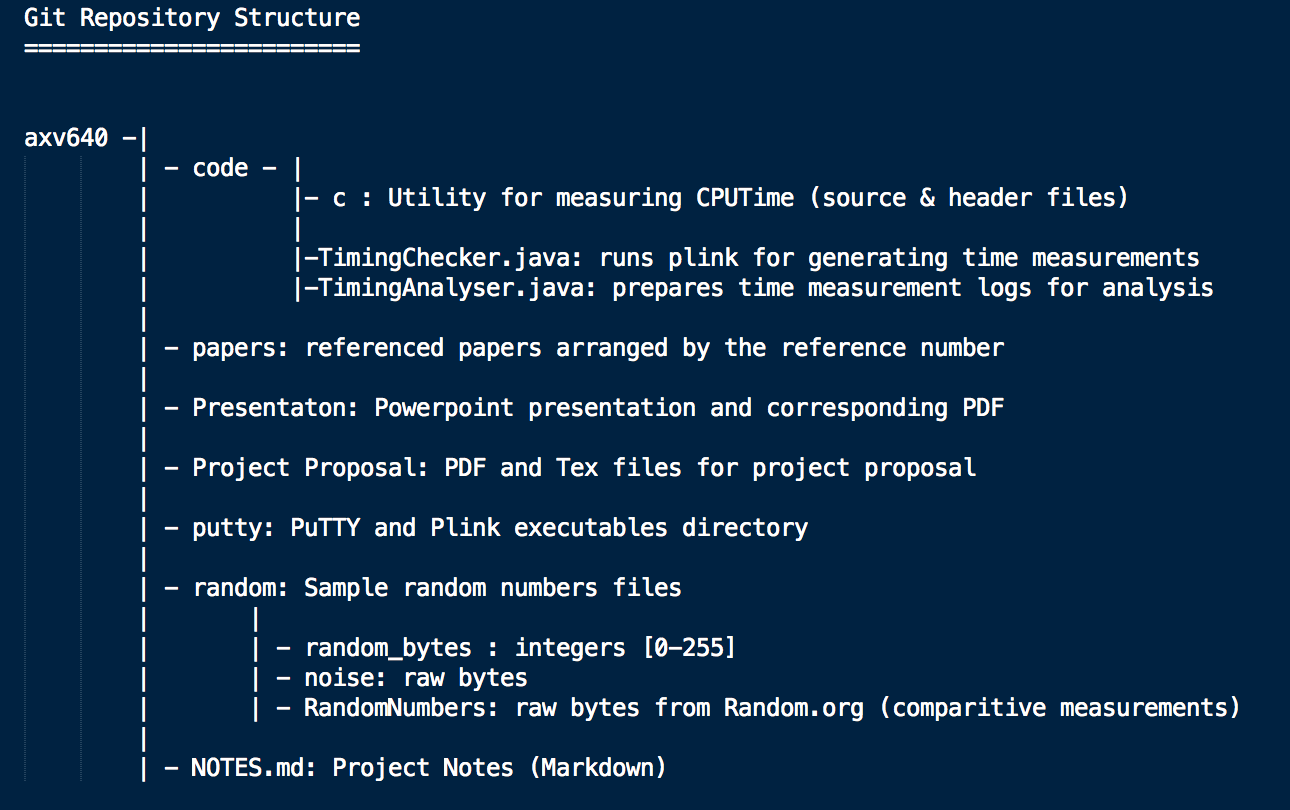
\includegraphics[width=1\textwidth]{RepoStructure.png}
\end{figure}
\chapter{Software and Tools}
List of Software and Tools used for the project along with their version details.
\begin{enumerate}
    \item Raspberry Pi machine (Raspbian-5+deb8u3)
    \item OpenSSH server running on Raspberry Pi (v6.7p1)
    \item Bitvise SSH Server (v7.33)
    (\url{https://www.bitvise.com/ssh-server-download})
    \item Microsoft Visual Studio Community 2017 (v15.2 26430.13 Release)
    \item Plink - For automated runs of PuTTY (v0.69) (\url{https://www.chiark.greenend.org.uk/~sgtatham/putty/})
    \item PuTTYgen - For RSA/DSA key generation (v0.69) (\url{https://www.chiark.greenend.org.uk/~sgtatham/putty/})
    \item CPUTime - Nadeau Software Consulting, Dr. David R. Nadeau: For measuring CPU Time (\url{http://nadeausoftware.com/articles/2012/03/c_c_tip_how_measure_cpu_time_benchmarking})
    \item ENT - Fourmilab: Pseudorandom number sequence test program (\url{http://www.fourmilab.ch/random/})
     \item Random.org - For generating random numbers for comparitive tests and as a reference for random number analysis. (\url{https://www.random.org})
    \item Wireshark (v2.4.0) (\url{https://www.wireshark.org/})
\end{enumerate}
\end{appendices}
\begin{thebibliography}{9}
\bibitem{putty}
PuTTY
\url{https://www.chiark.greenend.org.uk/~sgtatham/putty/}
\bibitem{rfc4251}
RFC 4251, The Secure Shell (SSH) Protocol Architecture,\\
\url{https://tools.ietf.org/html/rfc4251}
\bibitem{rfc4252}
RFC 4252, The Secure Shell (SSH) Authentication Protocol,\\  \url{https://tools.ietf.org/html/rfc4252}
\bibitem{rfc4253}
RFC 4253, The Secure Shell (SSH) Transport Layer Protocol,\\ \url{https://tools.ietf.org/html/rfc4253}
\bibitem{rfc4254}
RFC 4254, The Secure Shell (SSH) Connection Protocol,\\ \url{https://tools.ietf.org/html/rfc4254}
\bibitem{kocher96}
Paul C. Kocher, Timing Attacks on Implementations of Diffie-Hellman, RSA, DSS  and Other Systems. Annual International Cryptology Conference, Advances in Cryptology, CRYPTO' 96, pp 104-113
\bibitem{oorschot96}
On Diffie-Hellman Key Agreement with Short Exponents, Paul C. van Oorschot, Michael J. Wiener, International Conference on the Theory and Applications of Cryptographic Techniques, Advances in Cryptology — \\EUROCRYPT '96, pp 332-343
\bibitem{brumley}
Remote Timing Attacks are Practical, David Brumley, Dan Boneh, Computer Networks, Volume 48, Issue 5, 5 August 2005, Pages 701-716
\bibitem{adrian}
Imperfect Forward Secrecy: How Diffie-Hellman Fails in Practice, David Adrain et al.CCS '15, Proceedings of the 22nd ACM SIGSAC Conference on Computer and Communications Security
pp 5-17
\bibitem{randeval}
Randomness Evaluation Framework of Cryptographic Algorithms,Cristina-Loredana Duta, Bogdan-Costel Mocanu, Florin-Alexandru Vladescu,Laura Gheorghe,  
International Journal on Cryptography and Information Security (IJCIS), Vol. 4, No. 1, March 2014, \url{http://www.academia.edu/9902264/Randomness_Evaluation_Framework_of_Cryptographic_Algorithms}
\bibitem{foley}
Analysis of an On-line Random Number Generator, Louise Foley, April 2001, \url{https://www.random.org/analysis/Analysis2001.pdf}
\bibitem{garcia}
Make Sure DSA Signing Exponentiations Really are Constant-Time, Cesar Pereida García, Billy Bob Brumley, Yuval Yarom, Proceedings of the 2016 ACM SIGSAC Conference on Computer and Communications Security (CCS '16)
Pages 1639-1650
\bibitem{vadnala}
Attacking OpenSSL using Side-channel Attacks: the RSA case study, Praveen Kumar Vadnala, Lukasz Chmielewski, SHA2017,
\url{https://program.sha2017.org/system/event_attachments/attachments/000/000/038/original/sha_1_.pdf}
\end{thebibliography}
\listoffigures
\end{document}
